\subsubsection{Demonstrators}

\TOWRITE{NT}{Simulagora}

\TOWRITE{SL}{include the other demonstrators and emphasise links to rest of the project}

To confirm the usability of our software tools, and demonstrate their
value to potential academic and industrial users groups, we plan three
demonstrator projects. These will be developed as soon as the
necessary components are available to give early feedback and then
refined and maintained during the remainder of the project to
demonstrate the increasing scope and reliability of \TheProject.


\paragraph{Demonstrator: Interactive Books} ---
In \taskref{dissem}{ibook}  we will produce a series of interactive books
that can be read, executed, modified and explored within the
\TheProject VREs. This will demonstrate the collaboration and
document-handling capabilities of \TheProject and the ability to link
presentation to computation. The books will target students, an
audience familiar with modern web applications, but with traditional
computational tools. Evaluation of the acceptance of these books with
provide valuable feedback on our user interface components.

\begin{figure}
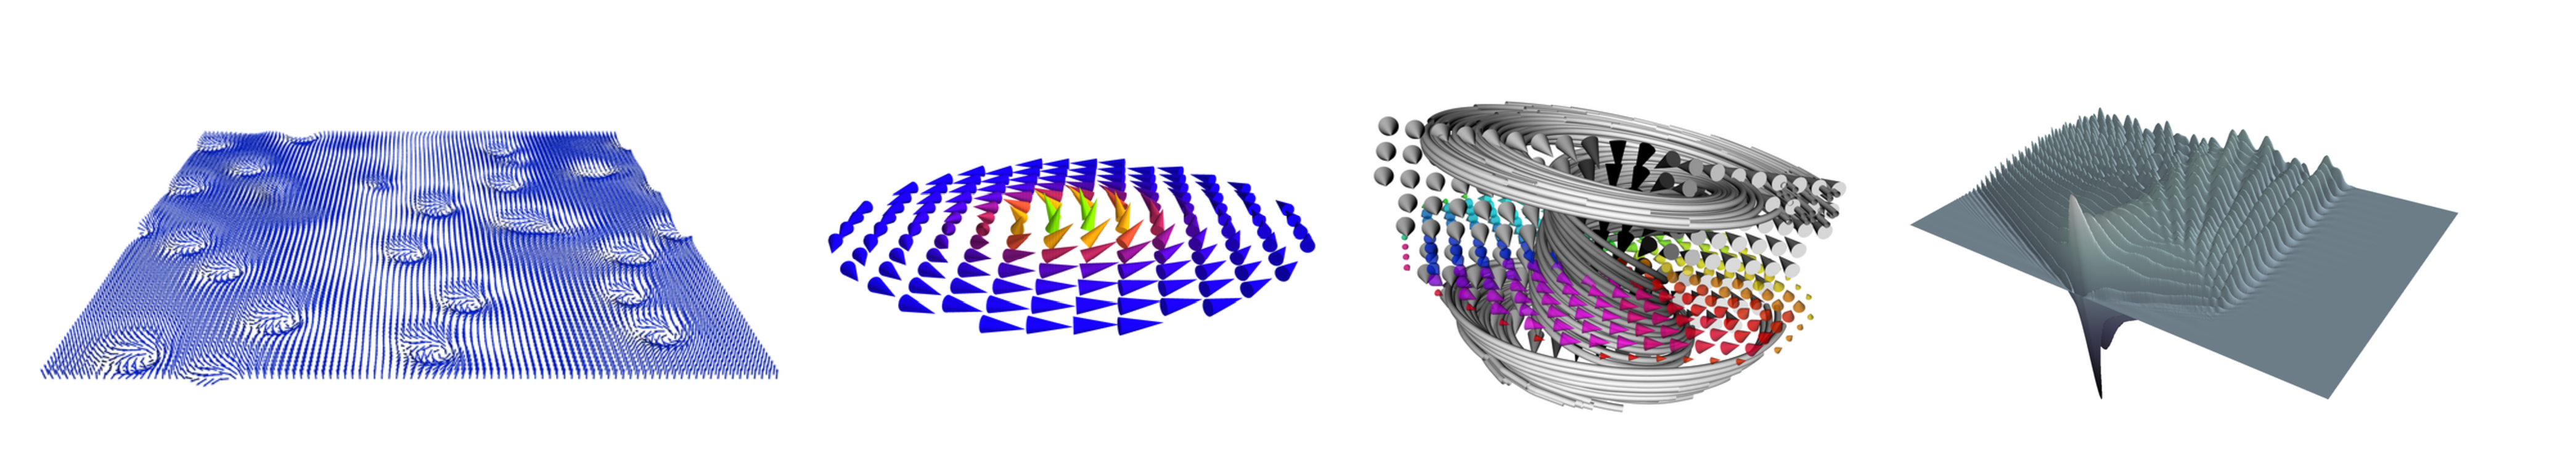
\includegraphics[width=1.0\textwidth]{Pictures/micromagnetic-and-3d-vis-4x1.pdf}
\caption{\label{fig:3d-plots} A selection of typical visualisation patterns often required in science and engineering. From left to right: a 3d vector field on a 2d domain, a 3d vector field coloured with another scalar field on a 2d domain, a 3d vectorfield on a 3d domain with streamlines, and scalar field plotted on a 2d domain.}
\end{figure}

\paragraph{Demonstrator: Micromagnetic VRE}
\label{sec:introduction-micromagnetic-vre-demonstrator} In
\taskref{UI}{oommf-py-ipython-attributes} we will build
a sample VRE targetting a specific research community, that of \textit{micromagnetics}.

Micromagnetics deals with the behaviour of
magnetisation at length scales of the order of
micrometers and below. It is widely used in the research and
development of magnetic data storage media and devices, for magnetic
sensing, permanent magnets and healthcare applications such as cancer
treatment and diagnostics. Figure~\ref{fig:3d-plots} shows some micromagnetic simulation results.
Researchers needing to carry out simulations in this area often do not
have  extensive computational background; they may be
material scientists, engineers and physicists that
interpreting  experiments and designing new devices. Industrial users include Seagate, Hitachi,
TDK, Samsung, Bosch and Toyota.


We will embed the most popular micromagnetic
simulation software (Object Oriented MicroMagnetic Framework
\cite{OOMMF-url}, which has over 1800 citations) within a micromagnetic VRE, complemented by other
components that add value, including notebook user interfaces,
replacing the current text driven, unautomated and error-prone workflow.

We will evaluate this demonstrator application in 
\taskref{social-aspects}{oommf-nb-evaluation}, immediately feeding
results back into the \TheProject work. This will also
be a case study for the sustainability of the approach and tool beyond
the life time of this H2020 project.

\paragraph{Demonstrator: Computational Mathematics Resource Indexing
Service}

In \taskref{dissem}{index-librorum-salvificorum} 
we will demonstrate the ability to build persistemnt highly-linked
web-based services using \TheProject by developing a unified index of
components and documents relevant to \TheProject. This will test
elements such as cloud interaction and internationalisation, and our
abvility to provide a uniform mathematical view of diverse
components. It will also serve
to advertise the range of components available.

